\documentclass{article}

\usepackage{listings} % for including MATLAB code
\usepackage{graphicx} % for including images

\title{80846 - Report - 1st}
\author{GU JUN, 6132230056-4}
\date{\today}

\begin{document}

\maketitle

\section*{Introduction}

The following content will be organized in the following way: Problem Statement, Simulink model, Source codes for RobotDynamics and controller blocks, Simulation results, and Explanation.

\section*{Problem Statement}

According to the class, we are required to complete two things: \\
\textbf{1. Robot dynamics with gravity.} \\
\textbf{2. PID controller with integration gain.}

% model of the system
\section{Simulink Model}
See the Figure \ref{fig:model} below. The whole system inclues two blocks: RobotDynamics and Controller.
And some integration and derivative blocks are used to calculate the error, derror, ierror and dq, q.
\begin{figure}[ht]
    \centering
    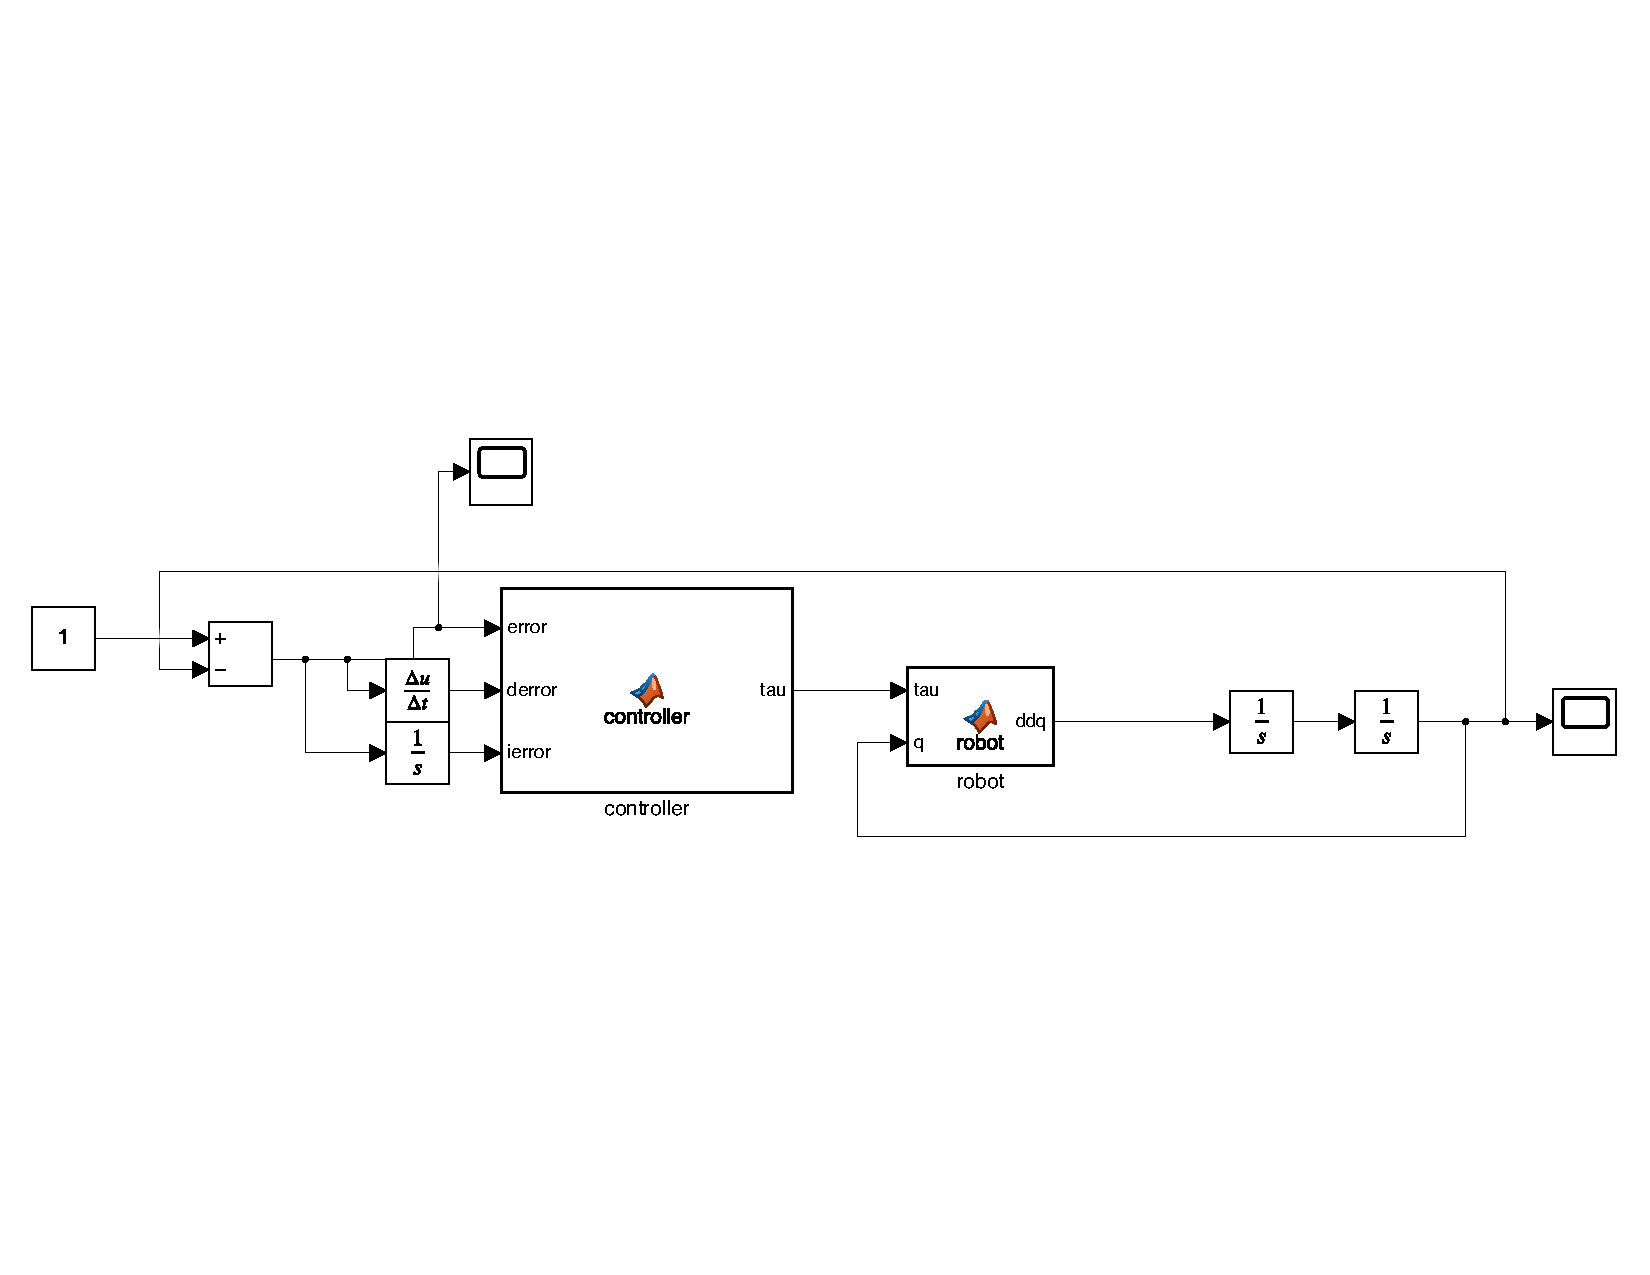
\includegraphics[width=0.9\textwidth]{figures/model.pdf}
    \caption{Simulink Model of whole system}
    \label{fig:model}
\end{figure}

% formulas and source codes
\section{Formulas and Source Codes}
This part inclues the formulas and source codes for RobotDynamics and Controller blocks.
\subsection*{RobotDynamics}
The robot dynamics is calculated by the following formula:
\begin{equation}
    \ddot{q} = \frac{\tau - m \cdot g \cdot \cos(q)}{I + m \cdot l_g \cdot l_g}
\end{equation}

where $I = 0.01$, $m = 0.5$, $l_g = 0.2$, $g = 9.8$ accoring to the problem setting.\\
\newpage
The source code is shown below:
\begin{lstlisting}[language=Matlab]
    function ddq = robot(tau, q)

        I = 0.01;
    
        m = 0.5;
    
        lg = 0.2;
    
        g = 9.8;
        % = 0;
        Ibar = I + m * lg * lg;
    
        tauBar = tau - m * g * lg * cos(q);
    
        ddq = tauBar / Ibar;
\end{lstlisting}

\subsection*{Controller}
The controller is calculated by the following formula:
\begin{equation}
    \tau = K_p \cdot error + K_d \cdot \frac{d}{dt}error + K_i \cdot \int_{0}^{\infty}error
\end{equation}
Because it is not easy to calculate the intgral and derivative in function, I calculate them in simulink model.\\
\break
The source code is shown below:
\begin{lstlisting}[language=Matlab]
    function tau = controller(error, derror, ierror)

        kp = 8;
    
        ki = 5;
    
        kd = 0.7;
    
        tau = kp * error + kd * derror + ki * ierror;
\end{lstlisting}

\section{Simulation Results}

After some tuning of the gains, I got the following Figure \ref{fig:result_plot}. The robot can reach the target position in a short time and the error is very small.\\

\begin{figure}[ht]
    \centering
    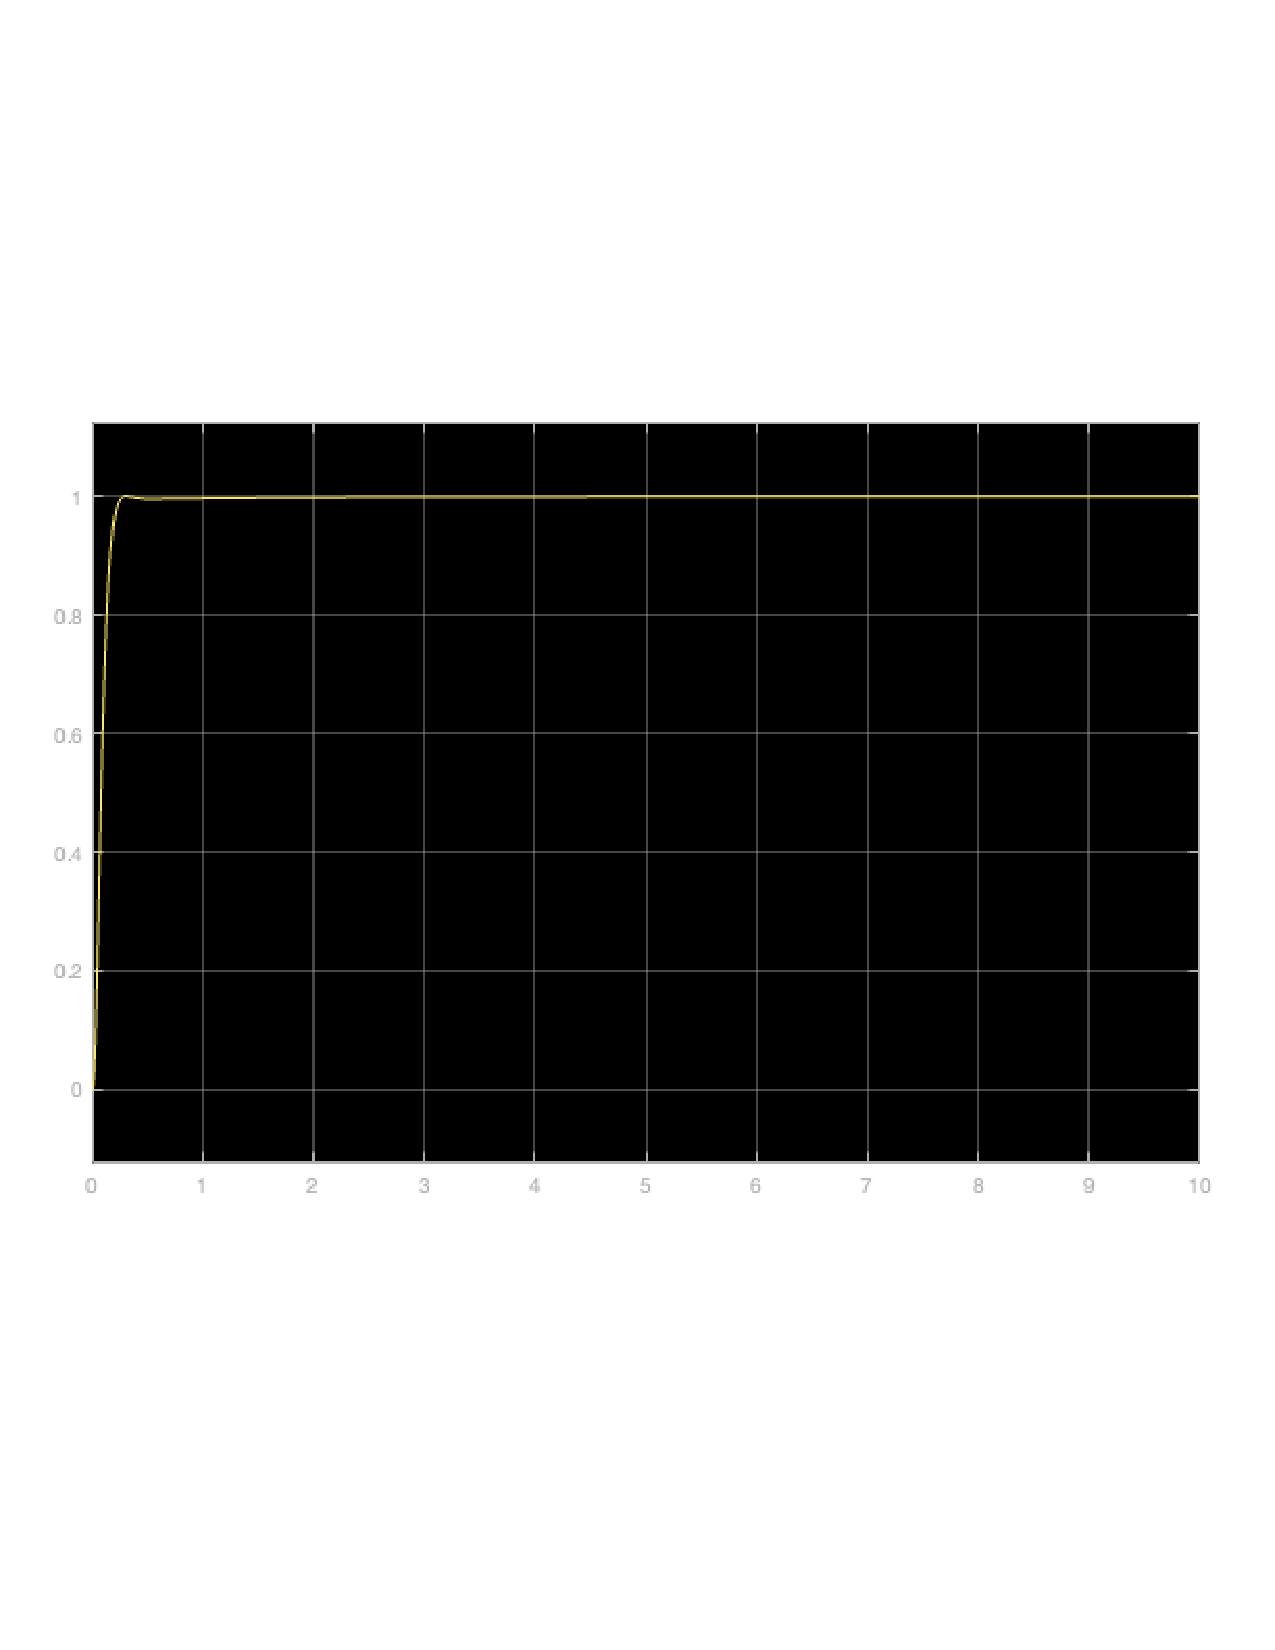
\includegraphics[width=0.8\textwidth]{figures/result.pdf}
    \caption{Result Plot, error disapear in 0.3 second.}
    \label{fig:result_plot}
\end{figure}

\section{Explanation}

According to the formulas and source codes, most parts are very clear. But there are some points need to be explained.\\
\textbf{1. Why the intgrals and derivatives all calculated outside} \\
Because it is not easy to calculate the intgral and derivative in function, you need a environment varible to store the previous values.\\
\textbf{2. Why the gains are set to 8, 5, 0.7} \\
I tried many times and found that these gains can make the robot reach the target position in a short time and the error is very small.\\
\end{document}